\documentclass[border=3pt]{standalone}
% Preâmbulo compartilhado pelos diagramas TikZ da aula 7 de Navegação (Implementação do A*)
\usepackage[T1]{fontenc}
\usepackage[utf8]{inputenc}
\usepackage{lmodern}
\usepackage{amsmath}
\usepackage{xcolor}
\usepackage{tikz}
\usetikzlibrary{arrows.meta,angles,quotes,decorations.pathmorphing,decorations.pathreplacing,calc,
                positioning,shapes.geometric,shapes.misc,backgrounds,fit,
                math}

% Paleta (mesma dos SVGs originais)
\definecolor{dblue}{HTML}{2A5B8C}
\definecolor{dorange}{HTML}{B3541E}
\definecolor{dgreen}{HTML}{4A7C59}
\definecolor{dred}{HTML}{9C4B4B}
\definecolor{dcream}{HTML}{F4F1EA}
\definecolor{dshade}{HTML}{DDD7C9}

% Função gaussiana (não normalizada por padrão de escala visual)
\pgfmathdeclarefunction{gauss}{3}{%
  \pgfmathparse{1/(#3*sqrt(2*pi))*exp(-((#1-#2)^2)/(2*#3^2))}%
}

% Estilos comuns (prefixo d... para não colidir com chaves internas do pgf)
\tikzset{
  >={Stealth[length=2mm]},
  dguide/.style={gray!55, dashed, line width=0.4pt},
  daxis/.style={gray!60, line width=0.7pt, ->},
  dbody/.style={fill=black!3, draw=black!80, line width=1pt},
  dacc/.style={draw=dblue, line width=1pt},
  dlbl/.style={black!55, font=\small},
  dsub/.style={black!45, font=\footnotesize},
  dstate/.style={circle, draw=black!80, fill=dcream, line width=1pt,
                 minimum size=17mm, font=\large, inner sep=1pt},
  dobs/.style={circle, draw=black!80, fill=dshade, line width=1pt,
               minimum size=14mm, font=\large, inner sep=1pt},
  dbox/.style={rounded corners=2pt, draw=black!80, fill=dcream, line width=1pt,
               align=center, inner sep=6pt},
  dop/.style={circle, draw=black!80, fill=white, line width=1pt,
              minimum size=6mm, inner sep=0pt, font=\small},
  dtrans/.style={->, dblue, line width=1pt},
  dmeas/.style={->, dorange, line width=1pt},
  dcurve/.style={line width=1pt, dblue},
  dcurveb/.style={line width=1.4pt, dorange},
}

\begin{document}
\hyphenpenalty=10000 \exhyphenpenalty=10000 \tolerance=9999 \emergencystretch=3em
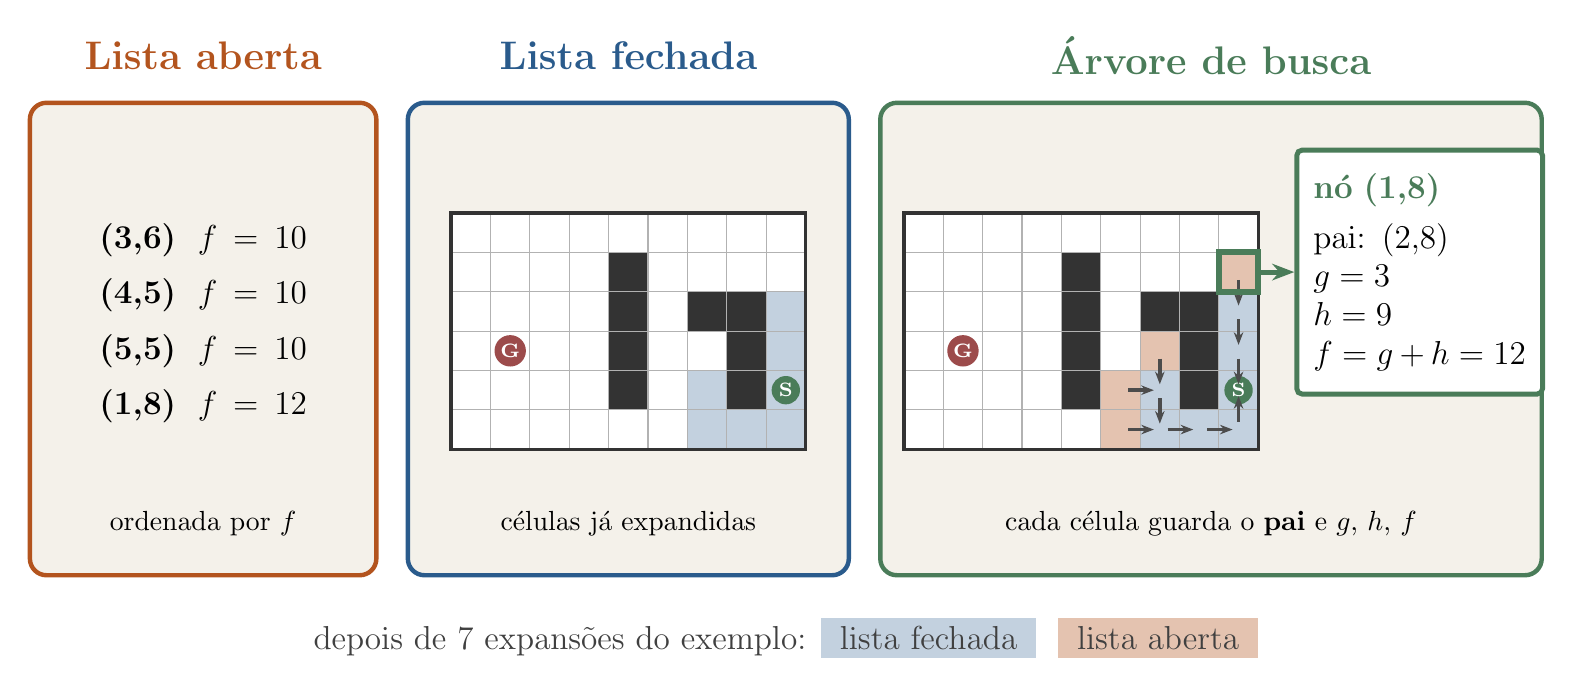
\begin{tikzpicture}[x=1cm,y=1cm]
\draw[dorange, line width=1.6pt, rounded corners=6pt, fill=dcream] (0.00,0.6) rectangle (4.40,6.6);
\node[font=\Large\bfseries, dorange] at (2.20,7.2) {Lista aberta};
\node[font=\normalsize, text width=4.0cm, align=center] at (2.20,1.25) {ordenada por $f$};
\draw[dblue, line width=1.6pt, rounded corners=6pt, fill=dcream] (4.80,0.6) rectangle (10.40,6.6);
\node[font=\Large\bfseries, dblue] at (7.60,7.2) {Lista fechada};
\node[font=\normalsize, text width=5.2cm, align=center] at (7.60,1.25) {células já expandidas};
\draw[dgreen, line width=1.6pt, rounded corners=6pt, fill=dcream] (10.80,0.6) rectangle (19.20,6.6);
\node[font=\Large\bfseries, dgreen] at (15.00,7.2) {Árvore de busca};
\node[font=\normalsize, text width=8.0cm, align=center] at (15.00,1.25) {cada célula guarda o \textbf{pai} e $g$, $h$, $f$};
\node[font=\large, text width=3.8cm, align=center] at (2.2,3.8) {\textbf{(3,6)} \ $f=10$\\[6pt] \textbf{(4,5)} \ $f=10$\\[6pt] \textbf{(5,5)} \ $f=10$\\[6pt] \textbf{(1,8)} \ $f=12$};
\draw[fill=white, draw=black!30, line width=0.4pt] (5.350,4.700) rectangle ++(0.500,0.500);
\draw[fill=white, draw=black!30, line width=0.4pt] (5.850,4.700) rectangle ++(0.500,0.500);
\draw[fill=white, draw=black!30, line width=0.4pt] (6.350,4.700) rectangle ++(0.500,0.500);
\draw[fill=white, draw=black!30, line width=0.4pt] (6.850,4.700) rectangle ++(0.500,0.500);
\draw[fill=white, draw=black!30, line width=0.4pt] (7.350,4.700) rectangle ++(0.500,0.500);
\draw[fill=white, draw=black!30, line width=0.4pt] (7.850,4.700) rectangle ++(0.500,0.500);
\draw[fill=white, draw=black!30, line width=0.4pt] (8.350,4.700) rectangle ++(0.500,0.500);
\draw[fill=white, draw=black!30, line width=0.4pt] (8.850,4.700) rectangle ++(0.500,0.500);
\draw[fill=white, draw=black!30, line width=0.4pt] (9.350,4.700) rectangle ++(0.500,0.500);
\draw[fill=white, draw=black!30, line width=0.4pt] (5.350,4.200) rectangle ++(0.500,0.500);
\draw[fill=white, draw=black!30, line width=0.4pt] (5.850,4.200) rectangle ++(0.500,0.500);
\draw[fill=white, draw=black!30, line width=0.4pt] (6.350,4.200) rectangle ++(0.500,0.500);
\draw[fill=white, draw=black!30, line width=0.4pt] (6.850,4.200) rectangle ++(0.500,0.500);
\draw[fill=black!80, draw=black!30, line width=0.4pt] (7.350,4.200) rectangle ++(0.500,0.500);
\draw[fill=white, draw=black!30, line width=0.4pt] (7.850,4.200) rectangle ++(0.500,0.500);
\draw[fill=white, draw=black!30, line width=0.4pt] (8.350,4.200) rectangle ++(0.500,0.500);
\draw[fill=white, draw=black!30, line width=0.4pt] (8.850,4.200) rectangle ++(0.500,0.500);
\draw[fill=white, draw=black!30, line width=0.4pt] (9.350,4.200) rectangle ++(0.500,0.500);
\draw[fill=white, draw=black!30, line width=0.4pt] (5.350,3.700) rectangle ++(0.500,0.500);
\draw[fill=white, draw=black!30, line width=0.4pt] (5.850,3.700) rectangle ++(0.500,0.500);
\draw[fill=white, draw=black!30, line width=0.4pt] (6.350,3.700) rectangle ++(0.500,0.500);
\draw[fill=white, draw=black!30, line width=0.4pt] (6.850,3.700) rectangle ++(0.500,0.500);
\draw[fill=black!80, draw=black!30, line width=0.4pt] (7.350,3.700) rectangle ++(0.500,0.500);
\draw[fill=white, draw=black!30, line width=0.4pt] (7.850,3.700) rectangle ++(0.500,0.500);
\draw[fill=black!80, draw=black!30, line width=0.4pt] (8.350,3.700) rectangle ++(0.500,0.500);
\draw[fill=black!80, draw=black!30, line width=0.4pt] (8.850,3.700) rectangle ++(0.500,0.500);
\draw[fill=dblue!28!white, draw=black!30, line width=0.4pt] (9.350,3.700) rectangle ++(0.500,0.500);
\draw[fill=white, draw=black!30, line width=0.4pt] (5.350,3.200) rectangle ++(0.500,0.500);
\draw[fill=white, draw=black!30, line width=0.4pt] (5.850,3.200) rectangle ++(0.500,0.500);
\draw[fill=white, draw=black!30, line width=0.4pt] (6.350,3.200) rectangle ++(0.500,0.500);
\draw[fill=white, draw=black!30, line width=0.4pt] (6.850,3.200) rectangle ++(0.500,0.500);
\draw[fill=black!80, draw=black!30, line width=0.4pt] (7.350,3.200) rectangle ++(0.500,0.500);
\draw[fill=white, draw=black!30, line width=0.4pt] (7.850,3.200) rectangle ++(0.500,0.500);
\draw[fill=white, draw=black!30, line width=0.4pt] (8.350,3.200) rectangle ++(0.500,0.500);
\draw[fill=black!80, draw=black!30, line width=0.4pt] (8.850,3.200) rectangle ++(0.500,0.500);
\draw[fill=dblue!28!white, draw=black!30, line width=0.4pt] (9.350,3.200) rectangle ++(0.500,0.500);
\draw[fill=white, draw=black!30, line width=0.4pt] (5.350,2.700) rectangle ++(0.500,0.500);
\draw[fill=white, draw=black!30, line width=0.4pt] (5.850,2.700) rectangle ++(0.500,0.500);
\draw[fill=white, draw=black!30, line width=0.4pt] (6.350,2.700) rectangle ++(0.500,0.500);
\draw[fill=white, draw=black!30, line width=0.4pt] (6.850,2.700) rectangle ++(0.500,0.500);
\draw[fill=black!80, draw=black!30, line width=0.4pt] (7.350,2.700) rectangle ++(0.500,0.500);
\draw[fill=white, draw=black!30, line width=0.4pt] (7.850,2.700) rectangle ++(0.500,0.500);
\draw[fill=dblue!28!white, draw=black!30, line width=0.4pt] (8.350,2.700) rectangle ++(0.500,0.500);
\draw[fill=black!80, draw=black!30, line width=0.4pt] (8.850,2.700) rectangle ++(0.500,0.500);
\draw[fill=dblue!28!white, draw=black!30, line width=0.4pt] (9.350,2.700) rectangle ++(0.500,0.500);
\draw[fill=white, draw=black!30, line width=0.4pt] (5.350,2.200) rectangle ++(0.500,0.500);
\draw[fill=white, draw=black!30, line width=0.4pt] (5.850,2.200) rectangle ++(0.500,0.500);
\draw[fill=white, draw=black!30, line width=0.4pt] (6.350,2.200) rectangle ++(0.500,0.500);
\draw[fill=white, draw=black!30, line width=0.4pt] (6.850,2.200) rectangle ++(0.500,0.500);
\draw[fill=white, draw=black!30, line width=0.4pt] (7.350,2.200) rectangle ++(0.500,0.500);
\draw[fill=white, draw=black!30, line width=0.4pt] (7.850,2.200) rectangle ++(0.500,0.500);
\draw[fill=dblue!28!white, draw=black!30, line width=0.4pt] (8.350,2.200) rectangle ++(0.500,0.500);
\draw[fill=dblue!28!white, draw=black!30, line width=0.4pt] (8.850,2.200) rectangle ++(0.500,0.500);
\draw[fill=dblue!28!white, draw=black!30, line width=0.4pt] (9.350,2.200) rectangle ++(0.500,0.500);
\draw[black!80, line width=1.2pt] (5.350,2.200) rectangle (9.850,5.200);
\node[circle, fill=dgreen, text=white, font=\bfseries\scriptsize, inner sep=1pt, minimum size=0.36cm] at (9.600,2.950) {S};
\node[circle, fill=dred, text=white, font=\bfseries\scriptsize, inner sep=1pt, minimum size=0.36cm] at (6.100,3.450) {G};
\draw[fill=white, draw=black!30, line width=0.4pt] (11.100,4.700) rectangle ++(0.500,0.500);
\draw[fill=white, draw=black!30, line width=0.4pt] (11.600,4.700) rectangle ++(0.500,0.500);
\draw[fill=white, draw=black!30, line width=0.4pt] (12.100,4.700) rectangle ++(0.500,0.500);
\draw[fill=white, draw=black!30, line width=0.4pt] (12.600,4.700) rectangle ++(0.500,0.500);
\draw[fill=white, draw=black!30, line width=0.4pt] (13.100,4.700) rectangle ++(0.500,0.500);
\draw[fill=white, draw=black!30, line width=0.4pt] (13.600,4.700) rectangle ++(0.500,0.500);
\draw[fill=white, draw=black!30, line width=0.4pt] (14.100,4.700) rectangle ++(0.500,0.500);
\draw[fill=white, draw=black!30, line width=0.4pt] (14.600,4.700) rectangle ++(0.500,0.500);
\draw[fill=white, draw=black!30, line width=0.4pt] (15.100,4.700) rectangle ++(0.500,0.500);
\draw[fill=white, draw=black!30, line width=0.4pt] (11.100,4.200) rectangle ++(0.500,0.500);
\draw[fill=white, draw=black!30, line width=0.4pt] (11.600,4.200) rectangle ++(0.500,0.500);
\draw[fill=white, draw=black!30, line width=0.4pt] (12.100,4.200) rectangle ++(0.500,0.500);
\draw[fill=white, draw=black!30, line width=0.4pt] (12.600,4.200) rectangle ++(0.500,0.500);
\draw[fill=black!80, draw=black!30, line width=0.4pt] (13.100,4.200) rectangle ++(0.500,0.500);
\draw[fill=white, draw=black!30, line width=0.4pt] (13.600,4.200) rectangle ++(0.500,0.500);
\draw[fill=white, draw=black!30, line width=0.4pt] (14.100,4.200) rectangle ++(0.500,0.500);
\draw[fill=white, draw=black!30, line width=0.4pt] (14.600,4.200) rectangle ++(0.500,0.500);
\draw[fill=dorange!35!white, draw=black!30, line width=0.4pt] (15.100,4.200) rectangle ++(0.500,0.500);
\draw[fill=white, draw=black!30, line width=0.4pt] (11.100,3.700) rectangle ++(0.500,0.500);
\draw[fill=white, draw=black!30, line width=0.4pt] (11.600,3.700) rectangle ++(0.500,0.500);
\draw[fill=white, draw=black!30, line width=0.4pt] (12.100,3.700) rectangle ++(0.500,0.500);
\draw[fill=white, draw=black!30, line width=0.4pt] (12.600,3.700) rectangle ++(0.500,0.500);
\draw[fill=black!80, draw=black!30, line width=0.4pt] (13.100,3.700) rectangle ++(0.500,0.500);
\draw[fill=white, draw=black!30, line width=0.4pt] (13.600,3.700) rectangle ++(0.500,0.500);
\draw[fill=black!80, draw=black!30, line width=0.4pt] (14.100,3.700) rectangle ++(0.500,0.500);
\draw[fill=black!80, draw=black!30, line width=0.4pt] (14.600,3.700) rectangle ++(0.500,0.500);
\draw[fill=dblue!28!white, draw=black!30, line width=0.4pt] (15.100,3.700) rectangle ++(0.500,0.500);
\draw[fill=white, draw=black!30, line width=0.4pt] (11.100,3.200) rectangle ++(0.500,0.500);
\draw[fill=white, draw=black!30, line width=0.4pt] (11.600,3.200) rectangle ++(0.500,0.500);
\draw[fill=white, draw=black!30, line width=0.4pt] (12.100,3.200) rectangle ++(0.500,0.500);
\draw[fill=white, draw=black!30, line width=0.4pt] (12.600,3.200) rectangle ++(0.500,0.500);
\draw[fill=black!80, draw=black!30, line width=0.4pt] (13.100,3.200) rectangle ++(0.500,0.500);
\draw[fill=white, draw=black!30, line width=0.4pt] (13.600,3.200) rectangle ++(0.500,0.500);
\draw[fill=dorange!35!white, draw=black!30, line width=0.4pt] (14.100,3.200) rectangle ++(0.500,0.500);
\draw[fill=black!80, draw=black!30, line width=0.4pt] (14.600,3.200) rectangle ++(0.500,0.500);
\draw[fill=dblue!28!white, draw=black!30, line width=0.4pt] (15.100,3.200) rectangle ++(0.500,0.500);
\draw[fill=white, draw=black!30, line width=0.4pt] (11.100,2.700) rectangle ++(0.500,0.500);
\draw[fill=white, draw=black!30, line width=0.4pt] (11.600,2.700) rectangle ++(0.500,0.500);
\draw[fill=white, draw=black!30, line width=0.4pt] (12.100,2.700) rectangle ++(0.500,0.500);
\draw[fill=white, draw=black!30, line width=0.4pt] (12.600,2.700) rectangle ++(0.500,0.500);
\draw[fill=black!80, draw=black!30, line width=0.4pt] (13.100,2.700) rectangle ++(0.500,0.500);
\draw[fill=dorange!35!white, draw=black!30, line width=0.4pt] (13.600,2.700) rectangle ++(0.500,0.500);
\draw[fill=dblue!28!white, draw=black!30, line width=0.4pt] (14.100,2.700) rectangle ++(0.500,0.500);
\draw[fill=black!80, draw=black!30, line width=0.4pt] (14.600,2.700) rectangle ++(0.500,0.500);
\draw[fill=dblue!28!white, draw=black!30, line width=0.4pt] (15.100,2.700) rectangle ++(0.500,0.500);
\draw[fill=white, draw=black!30, line width=0.4pt] (11.100,2.200) rectangle ++(0.500,0.500);
\draw[fill=white, draw=black!30, line width=0.4pt] (11.600,2.200) rectangle ++(0.500,0.500);
\draw[fill=white, draw=black!30, line width=0.4pt] (12.100,2.200) rectangle ++(0.500,0.500);
\draw[fill=white, draw=black!30, line width=0.4pt] (12.600,2.200) rectangle ++(0.500,0.500);
\draw[fill=white, draw=black!30, line width=0.4pt] (13.100,2.200) rectangle ++(0.500,0.500);
\draw[fill=dorange!35!white, draw=black!30, line width=0.4pt] (13.600,2.200) rectangle ++(0.500,0.500);
\draw[fill=dblue!28!white, draw=black!30, line width=0.4pt] (14.100,2.200) rectangle ++(0.500,0.500);
\draw[fill=dblue!28!white, draw=black!30, line width=0.4pt] (14.600,2.200) rectangle ++(0.500,0.500);
\draw[fill=dblue!28!white, draw=black!30, line width=0.4pt] (15.100,2.200) rectangle ++(0.500,0.500);
\draw[black!80, line width=1.2pt] (11.100,2.200) rectangle (15.600,5.200);
\node[circle, fill=dgreen, text=white, font=\bfseries\scriptsize, inner sep=1pt, minimum size=0.36cm] at (15.350,2.950) {S};
\node[circle, fill=dred, text=white, font=\bfseries\scriptsize, inner sep=1pt, minimum size=0.36cm] at (11.850,3.450) {G};
\draw[black!70, line width=1.3pt, -{Stealth[length=1.6mm]}] (15.350,3.350) -- (15.350,3.025);
\draw[black!70, line width=1.3pt, -{Stealth[length=1.6mm]}] (15.350,2.550) -- (15.350,2.875);
\draw[black!70, line width=1.3pt, -{Stealth[length=1.6mm]}] (15.350,3.850) -- (15.350,3.525);
\draw[black!70, line width=1.3pt, -{Stealth[length=1.6mm]}] (15.350,4.350) -- (15.350,4.025);
\draw[black!70, line width=1.3pt, -{Stealth[length=1.6mm]}] (14.950,2.450) -- (15.275,2.450);
\draw[black!70, line width=1.3pt, -{Stealth[length=1.6mm]}] (14.450,2.450) -- (14.775,2.450);
\draw[black!70, line width=1.3pt, -{Stealth[length=1.6mm]}] (14.350,2.850) -- (14.350,2.525);
\draw[black!70, line width=1.3pt, -{Stealth[length=1.6mm]}] (13.950,2.450) -- (14.275,2.450);
\draw[black!70, line width=1.3pt, -{Stealth[length=1.6mm]}] (14.350,3.350) -- (14.350,3.025);
\draw[black!70, line width=1.3pt, -{Stealth[length=1.6mm]}] (13.950,2.950) -- (14.275,2.950);
\draw[dgreen, line width=2.2pt] (15.100,4.200) rectangle ++(0.50,0.50);
\node[dbox, draw=dgreen, fill=white, line width=1.8pt, text width=2.7cm, minimum height=3.1cm, font=\large, align=left] (no) at (17.65,4.450) {\textbf{\textcolor{dgreen}{nó (1,8)}}\\[4pt] pai: (2,8)\\ $g=3$\\ $h=9$\\ $f=g+h=12$};
\draw[dgreen, line width=1.8pt, -{Stealth[length=2.8mm]}] (15.600,4.450) -- (no.west);
\node[font=\large, black!75] at (9.6,-0.2) {depois de 7 expansões do exemplo: \colorbox{dblue!28!white}{ lista fechada } \ \colorbox{dorange!35!white}{ lista aberta }};
\end{tikzpicture}
\end{document}
